\documentclass{article}
\usepackage[utf8]{inputenc}

\title{Converting Images To hand Drawn Sketches Using Novel Orthogonal Gaussian Lattice Method}
\author{Anish Sachdeva}
\date{November 2020}
\documentclass[titlepage]{article}

\usepackage{natbib}
\usepackage{graphicx}
\usepackage{algorithm}
\usepackage{algorithmic}
\usepackage[utf8]{inputenc}
\usepackage[top=2cm, bottom = 2cm, left=1.5cm, right=1.5cm ]{geometry}
\usepackage{amsfonts, amsmath, amssymb}
\usepackage[none]{hyphenat}
\usepackage{fancyhdr}
\usepackage{float}
\usepackage[nottoc, notlot, notlof]{tocbibind}
\usepackage{hyperref}
\usepackage{multicol}
\usepackage{subfig}
\usepackage{relsize}
\usepackage{xcolor}
\usepackage[colorlinks]{hyperref}

\pagestyle{fancy}
\fancyhead{}
\fancyfoot{}
\fancyhead[R]{\slshape }
\fancyfoot[c]{\thepage}
\renewcommand{\headrulewidth}{0.5pt}
\renewcommand{\footrulewidth}{0.5pt}

%This command is used to set the indentation of a paragraph
\parindent 0ex
\setlength{\parindent}{0em}
\renewcommand{\baselinestretch}{1.1}

\begin{document}

\begin{titlepage}
\begin{center}
\vspace*{1cm}
\vfill
\line(1,0){400}\\[1mm]
\huge{\textbf{Computer Graphics: Converting Images To hand Drawn Sketches Using Novel Orthogonal Gaussian Lattice Method}}\\[3mm]
\Large{\textbf{Anish Sachdeva}}\\[1mm]
\line(1,0){400}

\vfill  

\end{center}
\end{titlepage}


%Contents Page
\tableofcontents
\thispagestyle{empty}
\clearpage

\clearpage
\setcounter{page}{1}


\clearpage
\section{Introduction}
The problem that I have selected for this project is not something that is highly critical in nature or something that concerns our well being very much. It is also not something whose advancement will be very beneficial to us in terms of observable metrics. That is because the problem I have selected is that of creating a sketch composite from any given image $I$, such that the composite looks as if it was drawn by a sketch artist and not one created by a computer.\\

This problem is artistic in nature and hence can't be evaluated using a standard metric and the results given below have been produced using Hyperparameters tuned by me (so that the results look akin to something of my liking) and these hyperparameters can be changed and the results can be made to look to something of the users liking easily. \\

The key thing here are not the hyperparameters or results, but the method. This method gives excellent 
results not only for this application but is a completely new method of feature extraction from Images 
and can be used in several Applications. Some examples of other examples, more scientific in nature are 
given below in section 7 - $\textit{Future Scope}$. The project proposed there are of too great a length to 
be shown in all entirety here, hence a simple example of sketching has been selected to display the power 
of the Orthogonal Feature Extractor. \\

There are several ways of making a sketch from an Image. Below are examples of 3 different methods to 
produce a Sketch Composite from a given Image $I$. We study the different methods below and introduce the 
Orthogonal Gaussian Lattice Method and discuss trade-offs and benefits. \\

We observe in Figure 1 that the basic Canny edge Detection Algorithm although correctly identifies edges,
doesn't identify different gradients in different regions of the image and the results are too basic to
be declared sufficient for a sketch composite. \\

We observe from Figure 2 given below that the texture based method looks very much like the image itself 
and not at all like a hand drawn sketch. Furthermore the texture based method has a disadvantage that it 
changes the original image as it needs to clip away the image to convert it into the same aspect ratio as 
the texture. The Gaussian Blur Blend method in (c) gives much better results and doesn't need to change
the aspect ratio of the method, but the Gaussian Lattice Method in (d) gives considerable better results
overall and as this is art, personally looks the best of the bunch.

\begin{figure}[ht]
    \centering
    \subfloat[\centering Lenna: Standard Test Image]{{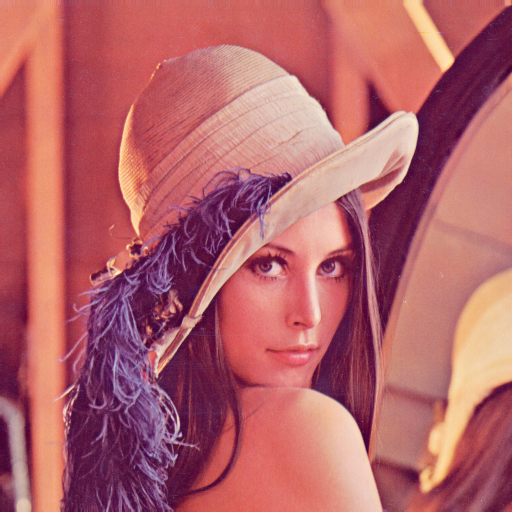
\includegraphics[height=8cm]{images/lenna/lenna.png} }}%
    \qquad
    \subfloat[\centering Sketch Composite Using Canny Edge Detection Method]{{\includegraphics[height=8cm]{images/lenna/canny-edge.png}}}%
    \caption{Sketch Composite of Standard Lenna Image Using Canny Edge Detection}
    \label{fig:lenna-canny-edge-detection}
\end{figure}

\begin{figure}[ht]
    \centering
    \subfloat[\centering Lenna: Standard Test Image]{{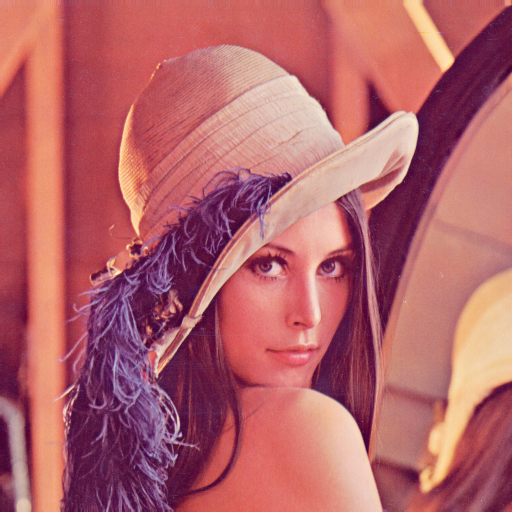
\includegraphics[height=8cm]{images/lenna/lenna.png} }}%
    \qquad
    \subfloat[\centering Sketch Composite Using Fixed Texture Application Method]{{\includegraphics[height=8cm]{images/lenna/texture.jpg}}}%
    \qquad
    \subfloat[\centering Sketch Composite Using Gaussian Blur and Blend Technique Image]{{\includegraphics[height=8cm]{images/lenna/lenna-blur-result.png} }}%
    \qquad
    \subfloat[\centering Sketch Composite Using Novel Method]{{\includegraphics[height=8cm]{images/lenna/lenna-result.png}}}%
    \caption{Different Methods to Convert Image to Sketch Composite}%
    \label{fig:lenna-different-methods}%
\end{figure}


\clearpage
\section{Basic Canny Edge Detection}
Canny Edge Detection as the name suggests is an algorithm to detect edges and is a very popular and 
robust algorithm used heavily in Computer Vision applications. It was developed by John F. Canny in 1986. 
\cite{canny-edge-detection}. Canny Edge Detection gives us the edges by computing the Gradient. \\

Since all edge detection results are easily affected by the noise in the image, it is essential to filter 
out the noise to prevent false detection caused by it. To smooth the image, a Gaussian filter kernel is 
convolved with the image. \\

\subsection{Gaussian Filtering}

This step will slightly smooth the image to reduce the effects of obvious noise 
on the edge detector. The equation for a Gaussian filter kernel of size (2k+1)×(2k+1) is given by:

\begin{equation*}
    H_{ij} = \frac{1}{2 \pi \sigma^2} \exp \left (\, - \frac{(i - (k + 1))^2 + (j - (k + 1))^2}{2 \sigma^2} \right )
\end{equation*} \\

Here is an example of a 5×5 Gaussian filter, used to create the adjacent image, with $\sigma  = 1$. (The asterisk denotes a convolution operation).

\begin{align*}
    B = \frac{1}{159}
    \begin{bmatrix}
        2 & 4 & 5 & 4 & 2 \\
        4 & 9 & 12 & 9 & 4 \\
        5 & 12 & 15 & 12 & 5 \\
        4 & 9 & 12 & 9 & 4 \\
        2 & 4 & 5 & 4 & 2 
    \end{bmatrix} * A
\end{align*} \\

It is important to understand that the selection of the size of the Gaussian kernel will affect the 
performance of the detector. The larger the size is, the lower the detector's sensitivity to noise. 
Additionally, the localization error to detect the edge will slightly increase with the increase of the 
Gaussian filter kernel size. A 5×5 is a good size for most cases, but this will also vary depending on 
specific situations. \\

\subsection{Finding The Intensity Gradient of The Image}
An edge in an image may point in a variety of directions, so the Canny algorithm uses four filters to 
detect horizontal, vertical and diagonal edges in the blurred image. The edge detection operator (such as 
Roberts, Prewitt, or Sobel) returns a value for the first derivative in the horizontal direction ($G_x$) 
and the vertical direction ($G_y$). From this the edge gradient and direction can be determined:

\begin{align*}
    G &= \sqrt{G_x^2 + G_y^2} \\
    \Theta &= \arctan{\frac{G_y}{G_x}}
\end{align*}

\subsection{The Algorithm}
The algorithm for performing canny edge Detection is given below. On my machine Intel Core i7-9750H CPU @
2.6 GHz with 16GB RAM and a Nvidia GeForce GTX 1650 GPU with 4GB of VRAM the following operation performed
in under 400 ms.

\begin{algorithm}
\caption{Canny Edge Detection Algorithm for a Given Image I}
    \begin{algorithmic}

    \STATE $kernel \leftarrow \text{5x5 Gaussian Kernel}$
    \STATE $I \gets I * kernel$
    
    \STATE \text{Create Sobel Kernel to calculate Image Derivatives $I_x$ and $I_y$} \\
    \STATE $k_x \leftarrow \begin{bmatrix}
        -1 & 0 & 1 \\
        -2 & 0 & 2 \\
        -1 & 0 & 1 
    \end{bmatrix}$
    
    \STATE $k_y \leftarrow \begin{bmatrix}
        1 & 2 & 1 \\
        0 & 0 & 0 \\
        -1 & 0 & 1 
    \end{bmatrix}$
    
    \STATE $\text{Compute the Derivatives $I_x$ and $I_y$ using $k_x$ and $k_y$}$
    \STATE $I_x \leftarrow I * k_x$
    \STATE $I_y \leftarrow I * k_y$
    
    \STATE \text{Compute Magnitude $G$ and angle $\Theta$ as}
    \STATE $G = \sqrt{I_x^2 + I_y^2}$
    \STATE $\Theta = \arctan{\frac{I_y}{I_x}}$
    
    \STATE \text{We now perform Non Maximum Suppression to reduce the variation in Edge Thickness}
    
    \FORALL{pixels $p$ in $I$}
        \FORALL{permitted angles $\theta$ in {$0^\circ$, $45^\circ$, $90^\circ$, $135^\circ$, $180^\circ$, $225^\circ$, $270^\circ$, $315^\circ$, $360^\circ$}}
            \STATE \text{Threshold all pixels with this gradient angle to 255 and the rest to 0}
        \ENDFOR
    \ENDFOR
    
    \STATE $result \gets I$
    \RETURN $result$
    \end{algorithmic}
\end{algorithm}

\subsection{Results}

Some results of Canny Edge Detection are given below:


\begin{figure}[ht]
    \centering
    \subfloat[\centering Original Image]{{\includegraphics[width=8cm]{images/butterfly/butterfly.jpg}}}%
    \qquad
    \subfloat[\centering Sketch Composite Using Canny Edge Detection] {{\includegraphics[width=8cm]{images/butterfly/canny-edge.png}}}%
    \caption{Canny Edge Detection Applied to Macro Image with Blurred Background}%
    \label{fig:canny-edge-detection-butterfly}%
\end{figure}

\begin{figure}[ht]
    \centering
    \subfloat[\centering Original Image]{{\includegraphics[width=8cm]{images/swiss-1/swiss-1.jpg}}}%
    \qquad
    \subfloat[\centering Sketch Composite Using Canny Edge Detection] {{\includegraphics[width=8cm]{images/swiss-1/canny-edge.png}}}%
    \caption{Canny Edge Detection Applied to Large Landscape Shot, with many Objects}%
    \label{fig:canny-edge-detection-swiss-1}%
\end{figure}

\begin{figure}[ht]
    \centering
    \subfloat[\centering Original Image]{{\includegraphics[width=8cm]{images/swiss-2/swiss-2.jpg}}}%
    \qquad
    \subfloat[\centering Sketch Composite Using Canny Edge Detection] {{\includegraphics[width=8cm]{images/swiss-2/canny-edge.png}}}%
    \caption{Canny Edge Detection Applied to Image with High Dynamic Range}%
    \label{fig:canny-edge-detection-swiss-2}%
\end{figure}

\begin{figure}[ht]
    \centering
    \subfloat[\centering Original Image]{{\includegraphics[width=8cm]{images/swiss-3/swiss-3.jpg}}}%
    \qquad
    \subfloat[\centering Sketch Composite Using Canny Edge Detection] {{\includegraphics[width=8cm]{images/swiss-3/canny-edge.png}}}%
    \caption{Canny Edge Detection Applied to Image with High Dynamic Range}%
    \label{fig:canny-edge-detection-swiss-3}%
\end{figure}

\begin{figure}[ht]
    \centering
    \subfloat[\centering Original Image]{{\includegraphics[width=8cm]{images/flower-rose/flower-rose.jpeg}}}%
    \qquad
    \subfloat[\centering Sketch Composite Using Canny Edge Detection] {{\includegraphics[width=8cm]{images/flower-rose/canny-edge.png}}}%
    \label{fig:canny-edge-detection-flower-rose}%
\end{figure}

\begin{figure}[ht]
    \centering
    \subfloat[\centering Original Image]{{\includegraphics[width=8cm]{images/flower-2/flower-2.jpg}}}%
    \qquad
    \subfloat[\centering Sketch Composite Using Canny Edge Detection] {{\includegraphics[width=8cm]{images/flower-2/canny-edge.png}}}%
    \label{fig:canny-edge-detection-flower-2}%
\end{figure}



\clearpage
\section{Fixed Texture Application For Creating Sketch Composite}
\subsection{Method}
In this method, we simply take a pre-defined texture file which is basically a mask that contains the pixel intensity values that should exist given an image $I$. Here the result produced will depend on the 
mask value of this texture file rather than the image $I$.

\subsection{Algorithm}
\begin{algorithm}
\caption{Applying Texture Mask on Image $I$}
    \begin{algorithmic}
    \REQUIRE The Image $I$
    \REQUIRE The mask $M$
    \STATE \text{Reshape the Image $I$ to match the ratio of $M$, crop the image if you must}
    \STATE $I \gets \text{Grayscale of I}$
    \STATE $result \gets I \cdot M$
    \RETURN $result$
    \end{algorithmic}
\end{algorithm}

\subsection{Results}
A few examples of sketch composites created using the fixed texture Application Method are given below:

\begin{figure}[ht]
    \centering
    \subfloat[\centering Original Image]{{\includegraphics[height=5cm]{images/butterfly/butterfly.jpg}}}%
    \qquad
    \subfloat[\centering Sketch Composite Using Simple Texture Application] {{\includegraphics[height=5cm]{images/butterfly/texture.jpg}}}%
    \label{fig:texture-butterfly}%
\end{figure}

\begin{figure}[ht]
    \centering
    \subfloat[\centering Original Image]{{\includegraphics[height=5cm]{images/dolphin/dolphin-2.jpg}}}%
    \qquad
    \subfloat[\centering Sketch Composite Using Simple Texture Application] {{\includegraphics[height=5cm]{images/dolphin/texture.jpg}}}%
    \label{fig:texture-dolphin-2}%
\end{figure}

\begin{figure}[ht]
    \centering
    \subfloat[\centering Original Image]{{\includegraphics[height=6cm]{images/flower-2/flower-2.jpg}}}%
    \qquad
    \subfloat[\centering Sketch Composite Using Simple Texture Application] {{\includegraphics[height=6cm]{images/flower-2/texture.jpg}}}%
    \label{fig:texture-flower-2}%
\end{figure}

\begin{figure}[ht]
    \centering
    \subfloat[\centering Original Image]{{\includegraphics[height=10cm]{images/flower-rose/flower-rose.jpeg}}}%
    \qquad
    \subfloat[\centering Sketch Composite Using Simple Texture Application] {{\includegraphics[height=10cm]{images/flower-rose/texture.jpg}}}%
    \label{fig:texture-flower-rose}%
\end{figure}

\begin{figure}[ht]
    \centering
    \subfloat[\centering Original Image]{{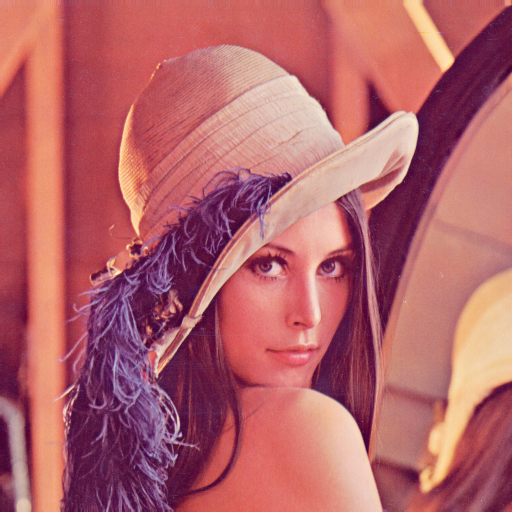
\includegraphics[height=7.5cm]{images/lenna/lenna.png}}}%
    \qquad
    \subfloat[\centering Sketch Composite Using Simple Texture Application] {{\includegraphics[height=7.5cm]{images/lenna/texture.jpg}}}%
    \label{fig:texture-lenna}%
    \caption{Texture Mask on Standard Lenna Image}
\end{figure}

\begin{figure}[ht]
    \centering
    \subfloat[\centering Original Image]{{\includegraphics[height=6cm]{images/swiss-1/swiss-1.jpg}}}%
    \qquad
    \subfloat[\centering Sketch Composite Using Simple Texture Application] {{\includegraphics[height=6cm]{images/swiss-1/texture.jpg}}}%
    \label{fig:texture-swiss-1}%
    \caption{Texture Mask on Swiss Landscape}
\end{figure}

\clearpage
\subsection{Conclusion}
We can clearly see from the above results that the result doesn't depend on any give Image but on the   
texture that we have selected. This is a computationally good method as it requires negligible time in 
applying a single texture filter, but the results don't seem very convincing and it doesn't seem as if
it were drawn by a human sketch artist. \\

Another disadvantage of using this method is that the texture may not be the same aspect ratio as the
given image and hence we either need to stretch out the texture to fit the image $I$ or we need to crop 
the image $I$ to fit to the texture. Changing the aspect ratio of the texture doesn't yield good results,
hence we always need to change the aspect ratio of the Image as can be seen above in the results. More
examples of this can be seen at \cite{photo-funia-sketch-effect}. \\

The results for some photos such as the Landscape Photograph in Figure 8 seem very good, but when we 
compare the same method for a portrait image such as Figure 7, we do not get good results and the 
result seems like a Sepia Photograph rather than a hand drawn sketch, so this method has a hit and miss
approach to this problem.

\clearpage
\section{Gaussian Blur Blend Technique For Creating Sketch Composite}
\subsection{Method}
This is a relatively straightforward method that borrows some techniques from the Canny Edge Detection 
Method, but rather than applying a Non Maximum Suppression in the Canny edge Detection, we will use a 
Dodge and Burn Blend Technique with our Gaussian Blur to obtain a sketch effect. \cite{gaussian-blend} \\

The steps are very simple, 

\begin{enumerate}
    \item Take the Image $I$.
    \item Take the Grayscale \cite{grayscale-image} of this Image $I$.
    \item Take the Negative of the grayscale obtained in step 2.
    \item Apply a Gaussian Blur \cite{gaussian-blur} to the Negative Obtained in Step 3.
    \item Blend the grayscale image from step 2 with the blurred negative from step 4 using a color dodge \cite{color-dodge}.
\end{enumerate}

\subsection{Gaussian Blur}

The Gaussian blur is a type of image-blurring filters that uses a Gaussian function (which also expresses the normal distribution in statistics) for calculating the transformation to apply to each pixel in the image. The formula of a Gaussian function in one dimension is

\begin{align*}
    G(x) = \frac{1}{\sigma \sqrt{2 \pi}} \exp \left( - \frac{x^2}{2 \sigma^2}\right)
\end{align*}

In two dimensions, it is the product of two such Gaussian functions, one in each dimension:

\begin{align*}
    G(x, y) = \frac{1}{2 \pi \sigma^2} \exp \left( - \frac{x^2 + y^2}{2 \sigma^2}\right)
\end{align*}

where $x$ is the distance from the origin in the horizontal axis, $y$ is the distance from the origin in 
the vertical axis, and $\sigma$ is the standard deviation of the Gaussian distribution. When applied in 
two dimensions, this formula produces a surface whose contours are concentric circles with a Gaussian 
distribution from the center point. \\

The time complexity of the Gaussian Blur Operation is $\mathcal{O} (w_{kernel} w_{image} h_{image}) + \mathcal{O} (h_{kernel} w_{image} h_{image})$. Gaussian Blur is a low pass filter attenuating high 
frequency signals.


\begin{figure}[ht]
    \centering
    \subfloat[\centering Standard Lenna Image with No Gaussian Blur]{{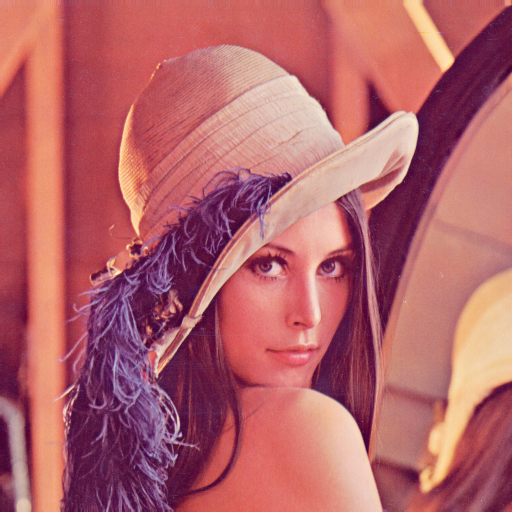
\includegraphics[width=3cm]{images/lenna/lenna.png}}}%
    \qquad
    \subfloat[\centering Gaussian Blur with $\sigma = 1$] {{\includegraphics[width=3cm]{images/lenna/gaussian-1.png}}}%
    \qquad
    \subfloat[\centering Gaussian Blur with $\sigma = 10$]{{\includegraphics[width=3cm]{images/lenna/gaussian-10.png}}}%
    \qquad
    \subfloat[\centering Gaussian Blur with $\sigma = 50$]{{\includegraphics[width=3cm]{images/lenna/gaussian-50.png}}}%
    \label{fig:lenna-gaussian-blur}%
    \caption{Gaussian Blur Applied to Lenna with Different Standard Deviations $\sigma$ and Kernel Size $k = (101, 101)$}
\end{figure}

\clearpage
\subsection{Color Dodge and Burn}
Dodging and burning are terms used in photography for a technique used during the printing process to  
manipulate the exposure of a selected area(s) on a photographic print, deviating from the rest of the 
image's exposure. In a darkroom print from a film negative, dodging decreases the exposure for areas of 
the print that the photographer wishes to be lighter, while burning increases the exposure to areas of the
print that should be darker. \\

Any material with varying degrees of opacity may be used, as preferred, to cover and/or obscure the 
desired area for burning or dodging. One may use a transparency with text, designs, patterns, a stencil, 
or a completely opaque material shaped according to the desired area of burning/dodging. \\

In both color doge and color burn we receive an Image $I$ and a mask $M$ and we use division operators
in images to obtain the dodge or burn using the mask we have. In the case of color doge the image
is brightened at the regions specified by the Mask. \\ 

In the following example we apply color dodge to standard Lenna Image using different Masks. We take 
same pixel value masks, where each pixel $p$ in the mask has the same value and the mask has dimensions
same as the image. \\

\begin{align*}
    M = \begin{bmatrix}
        p & p & p & \cdots & p \\
        p & p & p & \cdots & p \\
        \cdots \\
        \cdots \\
        p & p & p & \cdots & p
    \end{bmatrix}
\end{align*}

\begin{figure}[ht]
    \centering
    \subfloat[\centering Standard Lenna Image with No Color Dodge]{{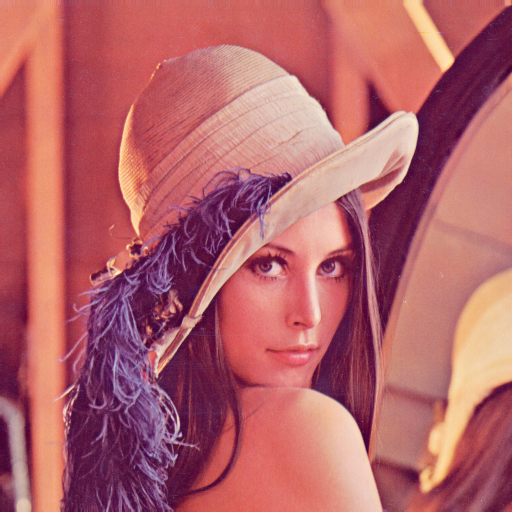
\includegraphics[width=3cm]{images/lenna/lenna.png}}}%
    \qquad
    \subfloat[\centering Color Dodge with $p = 100$] {{\includegraphics[width=3cm]{images/lenna/dodge-100.png}}}%
    \qquad
    \subfloat[\centering Color Dodge with $p = 150$]{{\includegraphics[width=3cm]{images/lenna/dodge-150.png}}}%
    \qquad
    \subfloat[\centering Color Dodge with $p = 200$]{{\includegraphics[width=3cm]{images/lenna/dodge-200.png}}}%
    \qquad
    \subfloat[\centering Color Dodge with $p = 254$]{{\includegraphics[width=3cm]{images/lenna/dodge-254.png}}}%
    \label{fig:lenna-gaussian-blur}%
    \caption{Color Dodge Applied to Lenna with Different Masks $M$ of constant dimensions, but different pixel values $p$.}
\end{figure}

\begin{figure}[ht]
    \centering
    \subfloat[\centering Standard Lenna Image with No Color Burn]{{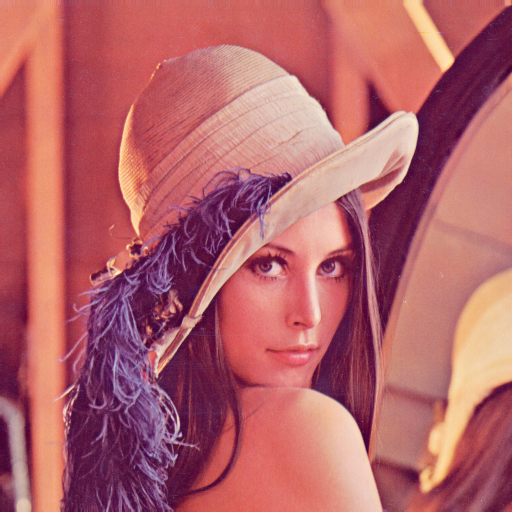
\includegraphics[width=3cm]{images/lenna/lenna.png}}}%
    \qquad
    \subfloat[\centering Color Burn with $p = 100$] {{\includegraphics[width=3cm]{images/lenna/burn-100.png}}}%
    \qquad
    \subfloat[\centering Color Burn with $p = 150$]{{\includegraphics[width=3cm]{images/lenna/burn-150.png}}}%
    \qquad
    \subfloat[\centering Color Burn with $p = 200$]{{\includegraphics[width=3cm]{images/lenna/burn-200.png}}}%
    \qquad
    \subfloat[\centering Color Burn with $p = 255$]{{\includegraphics[width=3cm]{images/lenna/burn-254.png}}}%
    \label{fig:lenna-gaussian-blur}%
    \caption{Color Burn Applied to Lenna with Different Masks $M$ of constant dimensions, but different pixel values $p$.}
\end{figure}


\clearpage
\subsection{Algorithm}
\begin{algorithm}
\caption{Creating the Sketch Composite from $I$ using Gaussian Blur and Blend Method}
    \begin{algorithmic}
    \REQUIRE The Image $I$
    \REQUIRE \textit{Sketch Density}: A Hyperparameter which will be used in The Gaussian Blurring Kernel Size and will decide the number of sketch lines to appear in the final result.
    \STATE \text{We create an Kernel of odd size, for convolution}
    \STATE $\text{Kernel Size} \gets 2 * (\textit{Sketch Density}, \textit{Sketch Density}) + 1$
    \STATE $J \gets$ Grayscale of Image $I$
    \STATE $B \gets$ Gaussian Blur of $J$ with kernel of size $k = \text{Kernel Size}$
    \STATE \text{We divide the Grayscale image with the Gaussian Blur of the Grayscale Image. The following is a pixel by pixel level}
    \STATE \text{operation which can be parallelized using a standard numerical matrix package.}
    \STATE $result \gets J / B$
    \RETURN $result$
    \end{algorithmic}
\end{algorithm}


\subsection{Results}
\begin{figure}[ht]
    \centering
    \subfloat[\centering Original Image]{{\includegraphics[width=8cm]{images/butterfly/butterfly.jpg}}}%
    \qquad
    \subfloat[\centering Sketch Composite Using Gaussian Blend Method] {{\includegraphics[width=8cm]{images/butterfly/blend.png}}}
    \caption{Gaussian Blur Blend Applied to Macro Butterfly Shot \label{fig:blend-butterfly}}
\end{figure}

\begin{figure}[ht]
    \centering
    \subfloat[\centering Original Image]{{\includegraphics[width=8cm]{images/dolphin/dolphin-2.jpg}}}%
    \qquad
    \subfloat[\centering Sketch Composite Using Gaussian Blend Method] {{\includegraphics[width=8cm]{images/dolphin/blend.png}}}%
    \caption{Gaussian Blur Blend Applied to Dolphin Photo with High Focus Shot \label{fig:blend-dolphin-2}}
\end{figure}

\begin{figure}[ht]
    \centering
    \subfloat[\centering Original Image]{{\includegraphics[width=8cm]{images/swiss-4/swiss-4.jpg}}}%
    \qquad
    \subfloat[\centering Sketch Composite Using Gaussian Blend Method] {{\includegraphics[width=8cm]{images/swiss-4/blend.png}}}%
    \caption{Gaussian Blur Blend Applied to Close Landscape Shot  \label{fig:blend-swiss-4}}
\end{figure}

\begin{figure}[ht]
    \centering
    \subfloat[\centering Original Image]{{\includegraphics[width=8cm]{images/flower-2/flower-2.jpg}}}%
    \qquad
    \subfloat[\centering Sketch Composite Using Gaussian Blend Method] {{\includegraphics[width=8cm]{images/flower-2/blend.png}}}%
    \caption{Gaussian Blur Blend Applied to Macro Photo With High Background Blur \label{fig:blend-flower-2}}
\end{figure}

\begin{figure}[ht]
    \centering
    \subfloat[\centering Original Image]{{\includegraphics[width=8cm]{images/flower-rose/flower-rose.jpeg}}}
    \qquad
    \subfloat[\centering Sketch Composite Using Gaussian Blend Method] {{\includegraphics[width=8cm]{images/flower-rose/blend.png}}}
    \caption{Gaussian Blur Blend Applied to Macro Flower Shot \label{fig:blend-flower-rose}}
\end{figure}

\begin{figure}[ht]
    \centering
    \subfloat[\centering Original Image]{{\includegraphics[width=8cm]{images/lenna/lenna.png}}}
    \qquad
    \subfloat[\centering Sketch Composite Using Gaussian Blend Method] {{\includegraphics[width=8cm]{images/lenna/lenna-blur-result.png}}}
    \caption{Gaussian Blur Blend Applied to Standard Lenna Portrait \label{fig:blend-lenna}}
\end{figure}

\begin{figure}[ht]
    \centering
    \subfloat[\centering Original Image]{{\includegraphics[width=8cm]{images/swiss-1/swiss-1.jpg}}}%
    \qquad
    \subfloat[\centering Sketch Composite Using Gaussian Blend Method] {{\includegraphics[width=8cm]{images/swiss-1/blend.png}}}
    \caption{Gaussian Blur Blend Applied to Swiss Landscape Shot \label{fig:blend-swiss-1}}
\end{figure}

\begin{figure}[ht]
    \centering
    \subfloat[\centering Original Image]{{\includegraphics[width=8cm]{images/swiss-2/swiss-2.jpg}}}
    \qquad
    \subfloat[\centering Sketch Composite Using Gaussian Blend Method] {{\includegraphics[width=8cm]{images/swiss-2/blend.png}}}
    \caption{\label{fig:blend-swiss-2}}
\end{figure}

\begin{figure}[ht]
    \centering
    \subfloat[\centering Original Image]{{\includegraphics[width=8cm]{images/swiss-3/swiss-3.jpg}}}
    \qquad
    \subfloat[\centering Sketch Composite Using Gaussian Blend Method] {{\includegraphics[width=8cm]{images/swiss-3/blend.png}}}
    \caption{\label{fig:blend-swiss-3}}
\end{figure}

\clearpage
\subsection{Conclusion}
We can see from the above Results that the results for Macro shots with low background noise or in many 
cases highly reduced blurred out background such as in Figure \ref{fig:blend-butterfly}, 
\ref{fig:blend-dolphin-2} and \ref{fig:blend-flower-2} the results are very good, especially for 
Figure \ref{fig:blend-butterfly}. \\

The same can't be said for the portrait photo of Lenna Figure-\ref{fig:blend-lenna}. This method does capture the
different edges part of the face, but the result seems like a Computer Generated Edge Map rather
a hand drawn sketch with different intensities. \\ 

Also for the landscape shots such as Figure-\ref{fig:blend-swiss-1}, Figure-\ref{fig:blend-swiss-2} and
Figure-\ref{fig:blend-swiss-3} the results are not very good. The method has successfully captured all
the various edges in the objects present, but there is no gradient in the image. There are no regions 
of the image where the pencil intensity is waxing and waning. Especially in the Bridge scene in 
Figure-\ref{fig:blend-swiss-4} the bridge lines seem very dark as compared to other lines and edges in
the image. Furthermore there is a soft shadow emanating from behind all the lines in all the images. \\

Notice especially Figure-\ref{fig:blend-flower-rose} where there is a very strong shadow behind the rose petals. This shadow is the result of the Gaussian Blur Blend Method and this shadow makes it appear 
computer generated rather than hand drawn. We can apply further filters and enhanced smoothing operators
such as the Laplacian smoothing operator, but these are specific methods trying to correct for specific bias in a few cases. Also that would still not correct for the very dark regions and strong edge detection
in particular regions. We now introduce a novel Feature Extraction Framework that can be used in countless
feature extraction tasks including Sketch Composite of an Image.


\clearpage
\section{Novel Method Using Orthogonal Gaussian Lattice}
View full project and further results at \underline{\href{https://github.com/anishLearnsToCode/image2sketch}{github.com/anishLearnsToCode/image-2-sketch}} \\

There are several regions in an Image, initial observation gives us the major features such as cars, 
people, the road, streets, bicycles, the footpath etc. If we observe closely we can identify softer 
features such as the lines on a person's face, or the strands of gray hair on the hair of a person. There 
are many different such features present in an Image and the following method is proposed.

\begin{enumerate}
    \item We Take 3 different Gaussian with different mean $\mu$ and std. deviation $\sigma$.
    \item We compute the Grayscale of the Image $I$, therefore reducing the Image pixel value from 3-dimensional to 1 dimensional.
    \item We normalize the pixel values in our grayscale Image.
    \item We compute 3 Gaussian Inverses using the 3 different Gaussian we took initially from the grayscale Image.
    \item Using the Gaussian Inverses we computed, we now take a sliding window of size $w$ and compute deviation spread Vectors (explained later) between a central and surrounding pixel.
    \item We take 3 different bounds, denoted in this project by $\alpha$ for the 3 different Gaussian.
    \item We compute 3 Simple Graphs from the 3 Gaussian Inverse using the deviation spread vectors and connectivity parameters $\alpha$ we took in step 6.
    \item We compute the Different Components in the 3 different Simple Graphs that we calculated in Step 7 and the separate components in a single Frame (Simple Graph) is called a Lattice.
    \item We can vary the type of lattices we create, the density of lattices and change the different features we discover by changing our 3 initial Gaussian that we select and also changing the connectivity bound parameter $\alpha$.
\end{enumerate}

\subsection{Grayscale of Image $I$}
An Image $I$ is defined as a function of 2 space coordinates $x$ and $y$ if we assume the image to be a 
discrete function with 2 axes. This can be denoted as $I = f(x, y)$ and each pixel is denoted by 3 distinct values denoting the amount of red, green and blue in the pixel. So each pixel can be denoted
by a 3 dimensional vector $(r, g, b)$. When we convert a RGB Image into grayscale, for every pixel we assign a single gray value between $0$ and $255$. \\

We compute Gray Value using the following method \cite{grayscale-image}:

\begin{align*}
    \text{Grayscale Image}(x, y) = 0.2126 \cdot R_{linear} + 0.7152 \cdot G_{linear} + 0.0722 \cdot B_{linear}
\end{align*}

\begin{figure}[ht]
    \centering
    \subfloat[\centering Original Image]{{\includegraphics[width=3cm]{images/lenna/lenna.png}}}
    \qquad
    \subfloat[\centering Grayscale of Image] {{\includegraphics[width=3cm]{images/lenna/grayscale.png}}}
    \qquad
    \caption{RGB $\rightarrow$ Grayscale for Lenna Image \label{fig:lenna-gaussian-inverse}}
\end{figure}

\subsection{Gaussian Inverse}
A standard Gaussian is defined as  
\begin{align*}
    G(x ; \mu, \sigma) = \frac{1}{\sigma \sqrt{2 \pi}} \exp \left( - \frac{1}{2} \left( \frac{x - \mu}{\sigma}\right) ^2 \right)
\end{align*}

where $\mu$ is the mean and $\sigma$ the standard deviation of the curve. The Gaussian Inverse which 
computes $x$ given $y$ is hence defined as (we are taking the positive $x$ branch in the formula below).

\begin{align*}
    G^{-1}(y ; \mu, \sigma) = \sigma * \sqrt{-2 * \log(y \sigma \sqrt{2 \pi}}) + \mu
\end{align*}

If we are given an image which is represented by a 2-dimensional Matrix $I$, we can compute the Gaussian Inverse of the image, which implies we calculate Gaussian Inverse of all pixel values separately. This can be parallelized using numerical Matrix library. The maximum value of the Gaussian Curve is at $x = \mu$, where $G(x = \mu ; \mu, \sigma) = \frac{1}{\sigma \sqrt{2 \pi}}$. \\

If we take a Gaussian with high standard deviation than that would imply that not all values would have an
inverse and any value larger than $\frac{1}{\sigma \sqrt{2 \pi}}$ would not have an inverse, so one of our 3 Gaussian should have $\sigma = \frac{1}{\sqrt{2 \pi}}$ so that for this Gaussian inverse exists for all 
$y \in [0, 1]$. \\

This formula is defined as follows for the computer, as we need to deal with imaginary quantities.

\begin{align*}
    G^{-1}(y ; \mu, \sigma) = \mu + \begin{cases}
        0 & y > \frac{1}{\sigma \sqrt{2 \pi}} \\
        \sigma * \sqrt{-2 * \log(y \sigma \sqrt{2 \pi}}) & \text{otherwise}
    \end{cases}
\end{align*}

Let us take 3 Gaussian as 

\begin{align*}
    G_1 \gets (\epsilon, \frac{4}{\sqrt{2 \pi}}) \\
    G_1 \gets (\epsilon, \frac{2}{\sqrt{2 \pi}}) \\
    G_1 \gets (\epsilon, \frac{1}{\sqrt{2 \pi}})
\end{align*}

where $\epsilon$ is a very small quantity, $10^{-5}$ in my program. The purpose of such a small quantity is 
for deviation spread ratio smoothing, which is explained later on. \\

We now compute the Gaussian  Inverse of Grayscale Images, for the first 2 Gaussian $G_1$ and $G_2$, not all values will have an inverse and for such values the pixel values will be represented as 0, for others
we will see valid values. So, the Gaussian Inverse will act as a mask for weeding out undesired high
pixel values and will also give us a non-polynomial smooth curve for feature extraction. \\

Pixel values exist in the range $p \in (0, 1, 2, \cdots ,255)$ (8-bit) where $p \in \mathbb{N}$. If we  
take a very high mean $\mu$, then our inverse function will give many values over 1, resulting in them 
being thresholded down to 255 and hence having a mean larger than $\mu > 0$ serves no purpose.

\begin{figure}[ht]
    \centering
    \subfloat[\centering Original Image]{{\includegraphics[width=2.5cm]{images/lenna/lenna.png}}}
    \qquad
    \subfloat[\centering Grayscale of Image] {{\includegraphics[width=2.5cm]{images/lenna/grayscale.png}}}
    \qquad
    \subfloat[\centering Gaussian Inverse of Grayscale with $\sigma = \frac{4}{\sqrt{2 \pi}}$] {{\includegraphics[width=2.5cm]{images/lenna/gaussian-inverse-4.0.png}}}
    \qquad
    \subfloat[\centering Gaussian Inverse of Grayscale with $\sigma = \frac{2}{\sqrt{2 \pi}}$] {{\includegraphics[width=2.5cm]{images/lenna/gaussian-inverse-2.0.png}}}
    \qquad
    \subfloat[\centering Gaussian Inverse of Grayscale with $\sigma = \frac{1}{\sqrt{2 \pi}}$] {{\includegraphics[width=2.5cm]{images/lenna/gaussian-inverse-1.0.png}}}
    \caption{Gaussian Inverse of Grayscale Lenna Image with different Gaussian Parameters $G_1$, $G_2$ and $G_3$\label{fig:lenna-gaussian-inverse}}
\end{figure}

\begin{figure}[ht]
    \centering
    \subfloat[\centering Original Image]{{\includegraphics[width=2.5cm]{images/dolphin/dolphin-2.jpg}}}
    \qquad
    \subfloat[\centering Grayscale of Image] {{\includegraphics[width=2.5cm]{images/dolphin/grayscale.png}}}
    \qquad
    \subfloat[\centering Gaussian Inverse of Grayscale with $\sigma = \frac{4}{\sqrt{2 \pi}}$] {{\includegraphics[width=2.5cm]{images/dolphin/gaussian-inverse-4.0.png}}}
    \qquad
    \subfloat[\centering Gaussian Inverse of Grayscale with $\sigma = \frac{2}{\sqrt{2 \pi}}$] {{\includegraphics[width=2.5cm]{images/dolphin/gaussian-inverse-2.0.png}}}
    \qquad
    \subfloat[\centering Gaussian Inverse of Grayscale with $\sigma = \frac{1}{\sqrt{2 \pi}}$] {{\includegraphics[width=2.5cm]{images/dolphin/gaussian-inverse-1.0.png}}}
    \caption{Gaussian Inverse of Grayscale Dolphin Image with different Gaussian Parameters $G_1$, $G_2$ and $G_3$\label{fig:dolphin-gaussian-inverse}}
\end{figure}

\begin{figure}[ht]
    \centering
    \subfloat[\centering Original Image]{{\includegraphics[width=2.5cm]{images/flower-rose/flower-rose.jpeg}}}
    \qquad
    \subfloat[\centering Grayscale of Image] {{\includegraphics[width=2.5cm]{images/flower-rose/grayscale.png}}}
    \qquad
    \subfloat[\centering Gaussian Inverse of Grayscale with $\sigma = \frac{4}{\sqrt{2 \pi}}$] {{\includegraphics[width=2.5cm]{images/flower-rose/gaussian-inverse-4.0.png}}}
    \qquad
    \subfloat[\centering Gaussian Inverse of Grayscale with $\sigma = \frac{2}{\sqrt{2 \pi}}$] {{\includegraphics[width=2.5cm]{images/flower-rose/gaussian-inverse-2.0.png}}}
    \qquad
    \subfloat[\centering Gaussian Inverse of Grayscale with $\sigma = \frac{1}{\sqrt{2 \pi}}$] {{\includegraphics[width=2.5cm]{images/flower-rose/gaussian-inverse-1.0.png}}}
    \caption{Gaussian Inverse of Grayscale Image with different Gaussian Parameters $G_1$, $G_2$ and $G_3$\label{fig:flower-rose-gaussian-inverse}}
\end{figure}

\clearpage
\subsection{Deviation Spread Ratio Vector}
We will now take a window of size $w$ ($w = 3$ in our program implementation) and will convolute the Image
$I$ with this window. In our window we will have a central pixel $p_x$ and surrounding pixels (8 in our case), which we denote by $p_s$.  \\

In every such window we will compute the ratio of surrounding pixels and the central pixel for the 8 possible surrounding pixel and central pixel pair. For 2 pixels in the window we will get 3 such ratios 
for the different Gaussian. Let us assume we have the following values for a $3 \times 3$ window of the
$3^d$ Gaussian.

\begin{align*}
    W = \begin{bmatrix}
        0.43 & 0.76 & 0.12 \\
        0.18 & 0.90 & 0.44 \\
        0.28 & 0.91 & 0.93
    \end{bmatrix}
\end{align*}


Taking the central pixel value as $0.90$, we get the 8 ratios as $\frac{p_s}{p_c}$  as:

\begin{align*}
    \begin{bmatrix}
        0.47 & 0.84 & 0.13 \\
        0.19 & - & 0.48 \\
        0.31 & 1.01 & 1.03
    \end{bmatrix}
\end{align*}

for every pixel pair $(p_s, p_c)$ we will get 3 such ratios for the 3 different Gaussian, which is what 
we will call the deviation ratio vector. These deviation ratios tell us different things. They are in fact the ratio of the z-score of the given pixel inverse values. In the Gaussian with smaller standard deviation $\sigma$ will have a lower ratio for the same amount of change in pixel values as compared to
the Gaussian with larger $\sigma$, where even a small change in values will trigger a large change in 
the deviation spread Ratio. So, the Gaussian with a larger $\sigma$ is being used to extract subtle 
features whereas the Gaussian with a smaller $\sigma$ is being used to extract regions of the image where
large changes will trigger a change in Ratio. \\

The 3 Different Gaussian are hence acting as an orthogonal Feature extraction mechanism where from the 
same pixel pair we are getting different ratios hence using the siding window technique we will get a
deviation spread ratio vector for every adjacent pixel pair in the image. \\

We will now use these deviation spreads to create 3 different Simple Graphs for the 3 Gaussian using 
the connectivity Parameters $<\alpha_i> \for i \in \{1, 2, 3\}$. Here $\alpha_i \in (0, 1]$.

\subsection{Lattices in Images}
We will consider every pixel in our image as a vertex, we will then compare the deviation spread ratio 
for very adjacent pixel with the connectivity parameter $\alpha$ for that particular Gaussian and if 
our ratio lies in the range $(\alpha, 1 / \alpha)$ then we will add an edge between these vertices. We will hence create 3 Simple Graphs for the 3 Gaussian and by varying the connectivity parameters $<\alpha_i>$, we can make our graph more or less connected and change the density of connected components.
In the first 2 Gaussian where not every pixel will have an inverse, if you recall we had chosen a small value $\epsilon$ for such pixels and this $\epsilon$ value will ensure that when we compute the ratio between any such pixels we do not encounter a Null value, but rather a number the computer can store. This step is what we call \underline{\textbf{Epsilon Smoothing}} and prevents underflow, overflow and Null values in actual program. \\

In our application and we will be proceeding by calling a single component in our Graph as a Lattice. 
Mathematically a Lattice is a connected, unweighted simple graph. Vertices inside a lattice actually represent a single pixel and have maximum degree 8 and minimum degree 0. The largest component possible
can be the size of the image and the smallest possible will be a trivial Lattice of size 1 pixel. \\

We can visualize different Lattices in Images by coloring each Lattice a Different Color and hence visualizing our Lattices. A tighter bound i.e $\alpha \rightarrow 1$ will produce many disconnected Lattices whereas a lenient bound $\alpha << 1$ will create a small number of large connected Lattices. Given below are a few examples: \textbf{\textit{(The colors are chosen at random for a lattice and have no significance)}}


\begin{figure}[ht]
    \centering
    \subfloat[\centering Original Image]{{\includegraphics[width=4cm]{images/lenna/lenna.png}}}
    \qquad
    \subfloat[\centering Lattices in Image with $G_1$ and $\alpha = 0.86$] {{\includegraphics[width=4cm]{images/lenna/0.86, 0.9, 0.94/lattice-0.png}}}
    \qquad
    \subfloat[\centering Lattices in Image with $G_2$ and $\alpha = 0.9$] {{\includegraphics[width=4cm]{images/lenna/0.86, 0.9, 0.94/lattice-1.png}}}
    \qquad
    \subfloat[\centering Lattices in Image with $G_3$ and $\alpha = 0.94$] {{\includegraphics[width=4cm]{images/lenna/0.86, 0.9, 0.94/lattice-2.png}}}
    \caption{Lattices in Different Simple Graphs with the connectivity parameter $<\alpha> = (0.86, 0.9, 0.94)$ \label{fig:lenna-lattice-color-0.86-0.9-0.94}}
\end{figure}

\begin{figure}[ht]
    \centering
    \subfloat[\centering Original Image]{{\includegraphics[width=4cm]{images/lenna/lenna.png}}}
    \qquad
    \subfloat[\centering Lattices in Image with $G_1$ and $\alpha = 0.98$] {{\includegraphics[width=4cm]{images/lenna/0.98, 0.98, 0.98/lattice-0.png}}}
    \qquad
    \subfloat[\centering Lattices in Image with $G_2$ and $\alpha = 0.98$] {{\includegraphics[width=4cm]{images/lenna/0.98, 0.98, 0.98/lattice-1.png}}}
    \qquad
    \subfloat[\centering Lattices in Image with $G_3$ and $\alpha = 0.98$] {{\includegraphics[width=4cm]{images/lenna/0.98, 0.98, 0.98/lattice-2.png}}}
    \caption{Lattices in Different Simple Graphs with the connectivity parameter $<\alpha> = (0.98, 0.98, 0.98)$ \label{fig:lenna-lattice-color-0.98-0.98-0.98}}
\end{figure}

\begin{figure}[h]
    \centering
    \subfloat[\centering Original Image]{{\includegraphics[width=4cm]{images/dolphin/dolphin-2.jpg}}}
    \qquad
    \subfloat[\centering Lattices in Image with $G_1$ and $\alpha = 0.86$] {{\includegraphics[width=4cm]{images/dolphin/0.86, 0.94, 0.98/lattice-0.png}}}
    \qquad
    \subfloat[\centering Lattices in Image with $G_2$ and $\alpha = 0.94$] {{\includegraphics[width=4cm]{images/dolphin/0.86, 0.94, 0.98/lattice-1.png}}}
    \qquad
    \subfloat[\centering Lattices in Image with $G_3$ and $\alpha = 0.98$] {{\includegraphics[width=4cm]{images/dolphin/0.86, 0.94, 0.98/lattice-2.png}}}
    \caption{Lattices in Different Simple Graphs with the connectivity parameter $<\alpha> = (0.86, 0.94, 0.98)$ \label{fig:dolphin-2-lattice-color-0.86-0.94-0.98}}
\end{figure}

\clearpage
\subsection{Lattice Vertex Coloring}
The above method to visualize the Lattices in the Images is a good method, but we have another method 
which will be the foundation for our sketching composite. The major problem we were facing with previous 
methods was there was no way to identify strong edges from lighter edges, and hence we could not make 
light and strong strokes as a real Human Sketch Artist will make. This issue can be resolved using the 
degree of pixels  (vertices) in our Simple Graph. \\

We know that every pixel must have at most a degree of 8 and in the trivial Lattice case, a degree of 0. 
This gives us 9 different degree values a pixel can have. Pixels that are heavily connected will lie deep 
inside a Lattice and Pixels that are at the border of the Lattice can at maximum be connected to 7 other 
pixels and would normally be connected to even less, normally 3-4. And completely isolated lattices will 
have a degree of 0. \\

We can assign different colors to pixels on the basis of their degree, where strongly connected pixels 
(degree 8) will have a white color and as the degree decreases, colors move towards Gray in the color 
spectrum. This will automatically give stronger edges a bolder color.

\begin{figure}[ht]
    \centering
    \subfloat[\centering Original Image]{{\includegraphics[width=4cm]{images/lenna/lenna.png}}}
    \qquad
    \subfloat[\centering Vertex Shading in $G_1$ with $\alpha = 0.86$] {{\includegraphics[width=4cm]{images/lenna/0.86, 0.9, 0.94/gaussian-0.png}}}
    \qquad
    \subfloat[\centering Vertex Shading in $G_2$ with $\alpha = 0.90$] {{\includegraphics[width=4cm]{images/lenna/0.86, 0.9, 0.94/gaussian-1.png}}}
    \qquad
    \subfloat[\centering Vertex Shading in $G_3$ with $\alpha = 0.94$] {{\includegraphics[width=4cm]{images/lenna/0.86, 0.9, 0.94/gaussian-2.png}}}
    \caption{Vertex Shading with Gaussian Parameters $G_1=(\epsilon, \frac{4}{\sqrt{2 \pi}}), G_1=(\epsilon, \frac{1.3}{\sqrt{2 \pi}}), G_1=(\epsilon, \frac{1}{\sqrt{2 \pi}})$ and $\alpha=(0.86, 0.9, 0.94)$ \label{fig:lenna-vertex-shading-(4, 1.3, 1)-(0.86, 0.9, 0.94)}}
\end{figure}

\begin{figure}[ht]
    \centering
    \subfloat[\centering Original Image]{{\includegraphics[width=4cm]{images/lenna/lenna.png}}}
    \qquad
    \subfloat[\centering Vertex Shading in $G_1$ with $\alpha = 0.86$] {{\includegraphics[width=4cm]{images/lenna/(4, 2, 1)-(0.86, 0.94, 0.98)/gaussian-0.png}}}
    \qquad
    \subfloat[\centering Vertex Shading in $G_2$ with $\alpha = 0.94$] {{\includegraphics[width=4cm]{images/lenna/(4, 2, 1)-(0.86, 0.94, 0.98)/gaussian-1.png}}}
    \qquad
    \subfloat[\centering Vertex Shading in $G_3$ with $\alpha = 0.98$] {{\includegraphics[width=4cm]{images/lenna/(4, 2, 1)-(0.86, 0.94, 0.98)/gaussian-2.png}}}
    \caption{\centering Vertex Shading with Gaussian Parameters $G_1=(\epsilon, \frac{4}{\sqrt{2 \pi}})$, $G_1=(\epsilon, \frac{2}{\sqrt{2 \pi}})$, $G_1=(\epsilon, \frac{1}{\sqrt{2 \pi}})$ and $\alpha=(0.86, 0.94, 0.98)$ \label{fig:lenna-vertex-shading-(4, 2, 1)-(0.86, 0.9, 0.94)}}
\end{figure}

\clearpage
\subsection{Linear Fusion of Orthogonal Gaussian Lattice Results with Standard Gaussian Blend}
We have seen in the results above that we are obtaining excellent shadings of different regions of the Image using our Vertex Shading Method of the different Gaussian Lattices, but we want only one image where all these different features our prominent. The simplest way to achieve this is taking a simple weighted average of our 3 Gaussian Vertex Shaded results and the Gaussian Blend Image Created in the above section (which is current State of The Art Method). To take a weighted average we assume a Hyperparameter $weight, W = (w_1, w_2, w_3, w_{gb})$ where $<w_i> \forall i \in \{1, 2, 3\}$ are for the 3 Gaussian and $w_{gb}$ is for the Gaussian Blend Method. Also, $\sum \lowerlimit_{w^{(i)} \in W} w^{(i)} = 1$. \\

The weight $w_3$ is most important as the $3^d$ Gaussian captures inverses of all Pixel values and acts as the base for the entire image. This weight $w_3$ is hence being treated as a hyper-parameter \textbf{Hand Drawn} which implies to the user how much hand drawn feel the user would like. High values like $[0.7, 1)$ would make it feel very sketchy and completely negate the Blend part, whereas lower values between $[0, 0.2]$ will make it feel more like the Gaussian-Blend result. The parameters \textit{Hand Drawn} and \textit{Sketch Density} are the 2 parameters the user will control to vary results.
 
\begin{align*}
    result = w_1 \cdot {VS}_1 + w_2 \cdot {VS}_2 + w_3 \cdot {VS}_3 + w_{gb} \cdot R_{gb} 
\end{align*}

\begin{figure}[ht]
    \centering
    \subfloat[\centering Original Image]{{\includegraphics[width=5.5cm]{images/lenna/lenna.png}}}
    \qquad
    \subfloat[\centering Weighted Result $W=(0.03, 0.03, 0, 0.94)$] {{\includegraphics[width=5.5cm]{images/lenna/(4, 2, 1)-(0.86, 0.94, 0.94)/novel-0.png}}}
    \qquad
    \subfloat[\centering Weighted Result $W=(0.03, 0.03, 0.15, 0.79)$] {{\includegraphics[width=5.5cm]{images/lenna/(4, 2, 1)-(0.86, 0.94, 0.94)/novel-0.15.png}}}
    \qquad
    \subfloat[\centering Weighted Result $W=(0.03, 0.03, 0.30, 0.64)$] {{\includegraphics[width=5.5cm]{images/lenna/(4, 2, 1)-(0.86, 0.94, 0.94)/novel-0.3.png}}}
    \qquad
    \subfloat[\centering Weighted Result $W=(0.03, 0.03, 0.45, 0.49)$] {{\includegraphics[width=5.5cm]{images/lenna/(4, 2, 1)-(0.86, 0.94, 0.94)/novel-0.45.png}}}
    \qquad
    \subfloat[\centering Weighted Result $W=(0.03, 0.03, 0.60, 0.34)$] {{\includegraphics[width=5.5cm]{images/lenna/(4, 2, 1)-(0.86, 0.94, 0.94)/novel-0.6.png}}}
    \caption{\centering Weighted Mean Results with Gaussian Parameters $G_1=(\epsilon, \frac{4}{\sqrt{2 \pi}}), G_1=(\epsilon, \frac{2}{\sqrt{2 \pi}}), G_1=(\epsilon, \frac{1}{\sqrt{2 \pi}})$ and $\alpha=(0.86, 0.94, 0.94)$ \label{fig:lenna-result-(4, 2, 1)-(0.86, 0.94 0.94)}}
\end{figure}

We can clearly see as we grow the hyper-parameter $w_3$, which is the \textbf{Hand Drawn} parameter, we get a much more sketch like looking Image. The results in Figure-\ref{fig:lenna-result-(4, 2, 1)-(0.86, 0.94 0.94)} image (b) is from the Gaussian Blur Blend Method, and the following results ; (c), (d), (e) and (f) are from the Orthogonal Gaussian Lattice Method and look distinctly better. A few other examples are:

\begin{figure}[ht]
    \centering
    \subfloat[\centering Original Image]{{\includegraphics[width=8.5cm]{images/dolphin/dolphin-2.jpg}}}
    \qquad
    \subfloat[\centering Weighted Result $W=(0, 0, 0, 1)$] {{\includegraphics[width=8.5cm]{images/dolphin/blend.png}}}
    \qquad
    \subfloat[\centering Weighted Result $W=(0, 0.1, 0.2, 0.7)$] {{\includegraphics[width=8.5cm]{images/dolphin/(4, 2, 1)-(0.86, 0.94, 0.94)/novel-(0, 0.1, 0.2).png}}}
    \qquad
    \subfloat[\centering Weighted Result $W=(0.1, 0.15, 0.3, 0.45)$] {{\includegraphics[width=8.5cm]{images/dolphin/(4, 2, 1)-(0.86, 0.94, 0.94)/novel-(0.1, 0.15, 0.3).png}}}
    \qquad
    \subfloat[\centering Weighted Result $W=(0.2, 0.1, 0, 0.7)$] {{\includegraphics[width=8.5cm]{images/dolphin/(4, 2, 1)-(0.86, 0.94, 0.94)/novel-(0.2, 0.1, 0).png}}}
    \qquad
    \subfloat[\centering Weighted Result $W=(0.2, 0.1, 0.2, 0.5)$] {{\includegraphics[width=8.5cm]{images/dolphin/(4, 2, 1)-(0.86, 0.94, 0.94)/novel-(0.2, 0.1, 0.2).png}}}
    \caption{\centering Weighted Mean Results with Gaussian Parameters $G_1=(\epsilon, \frac{4}{\sqrt{2 \pi}}), G_1=(\epsilon, \frac{2}{\sqrt{2 \pi}}), G_1=(\epsilon, \frac{1}{\sqrt{2 \pi}})$ with $\alpha=(0.86, 0.94, 0.94)$ and \textbf{Sketch Density} = 17\label{fig:dolphin-2-result-(4, 2, 1)-(0.86, 0.94 0.94)}}
\end{figure}

\clearpage
\subsection{Full Algorithm}
\begin{algorithm}
\caption{Calculating the Deviation vectors from a Given image I}
    \begin{algorithmic}
    \REQUIRE Image matrix I
    
    % Convert Image to gray scale
    \STATE I $\leftarrow$ grayscale(I)
    
    % Normalize the Image
    \STATE I $\leftarrow$ I / 255
    
    \text{We create 3 Gaussian}
    % Create 3 Gaussian
    \STATE $G_1 \leftarrow (\mu_1, \sigma_1)$
    \STATE $G_2 \leftarrow (\mu_2, \sigma_2)$
    \STATE $G_3 \leftarrow (\mu_3, \sigma_3)$
    
    \text{We compute the Inverse Gaussian of the Image with the 3 Gaussian}
    \STATE ${IG}_1 = InverseGaussian(I, G_1)$
    \STATE ${IG}_2 = InverseGaussian(I, G_2)$
    \STATE ${IG}_3 = InverseGaussian(I, G_3)$
    
    \STATE \text{We now create a 3 $\times$ 3 or $w \times w$ sliding window and slide over our image to compute the Deviation Vectors.}
    \STATE \text{The Deviation Vector of the surrounding and central Pixel Value are the ratio of}
    \STATE \text{the deviation spread if the 2 pixels with the 3 Gaussian.}
    
    \FORALL{windows $w$ in $I$}
        \FORALL{surrounding pixels $p_s$ in window $w$ for central pixel $p_c$}
            deviation($p_c$, $p_s$) = DeviationVector($p_c$, $p_s$, $IG_1$, $IG_2$, $IG_3$)
        \ENDFOR
    \ENDFOR
    
    \text{Here a single deviation vector is a $3 \times 1$ row vector}
    
    \RETURN DevaiationVectors as $D$
    \end{algorithmic}
\end{algorithm}

\begin{algorithm}
\caption{Computing the Simple Graphs from the Deviation Vectors $D$ and Connectivity Bounds $\alpha$}
    \begin{algorithmic}
    \REQUIRE Deviation vectors $D$
    \REQUIRE Connectivity Bounds $\alpha$
    \STATE \text{Create 3 Simple Graphs} $U_1$, $U_2$ \text{and} $U_3$ \text{with no. of vertices = number of pixels and no edges}
    
    \FORALL{deviation vectors $d^{(i)}$ in $D$}
        \FORALL{ratios $d^{(i)}_{j}$ in $d^{(i)}$}
            \IF{$d^{(i)}_{j}$ bounded by $(\alpha_j, {1 / \alpha}_j)$}
                \text{Add an edge between the pixels for this deviation vector $d^{(i)}$ in the Simple Graph $U_j$}
            \ENDIF
        \ENDFOR
    \ENDFOR
    
    \RETURN Simple Graphs $U_1$, $U_2$ and $U_3$
    \end{algorithmic}
\end{algorithm}

\begin{algorithm}
\caption{Computing the Lattices from the Graphs $U_1$, $U_2$ and $U_3$ using Standard Graph Theory Extracting Components List Algorithm}
    \begin{algorithmic}
    \REQUIRE Simple Graphs $U_1$, $U_2$ and $U_3$
    \STATE $L_1 \gets$ \text{lattices from}  $U_1$
    \STATE $L_2 \gets$ \text{lattices from}  $U_2$
    \STATE $L_3 \gets$ \text{lattices from}  $U_3$
    \RETURN Lattices $L_1$, $L_2$ and $L_3$
    \end{algorithmic}
\end{algorithm}

\begin{algorithm}
\caption{Computing Lattice Coloring Graph For the 3 Gaussian Based on The Lattices $L_1$, $L_1$ and $L_1$}
    \begin{algorithmic}
        \REQUIRE Lattices $L_1$, $L_2$ and $L_3$
        \STATE Create 3 new images for the results $J_1$, $J_2$ and $J_3$
        \FORALL{Gaussian lattices $L$ in $L_i$}
            \STATE Each Gaussian Lattices is a list of the several lattices for that particular Gaussian
            \FORALL{Lattice $l$ in $L$}
                \STATE \text{Each Lattice is a connected component in that particular Graph for a specific Gaussian}
                \STATE $pixelColor \gets Random Color()$
                \FORALL{pixels $p$ in Lattice $l$}
                    \STATE Assign pixel $p$ color $pixelColor$ in result image $J_i$
                \ENDFOR
            \ENDFOR
        \ENDFOR
        \RETURN Resulting Images $J_1$, $J_2$ and $J_3$
    \end{algorithmic}
\end{algorithm}

\begin{algorithm}
\caption{Computing The Vertex Shaded Image Given The Simple Graphs $U_i$ for different Gaussian for image $I$}
    \begin{algorithmic}
        \REQUIRE Image $I$
        \REQUIRE Simple Graphs $U_i$ for $\{1, 2, 3\}$ for the 3 Gaussian
        \STATE Create 3 new Images $J_1$, $J_2$ and $J_3$ which will be the result
        \FORALL{Simple Graph $U$ in $U_i$ and resulting Image $J$ in $J_i$}
            \FORALL{Vertices $v$ in $U$}
                \STATE \textit{pixel\_color} $\gets$ \textit{PixelColorFromDegree(v.degree)}
                \STATE Assign pixel $v$ in $J$ color \textit{pixel\_color}
            \ENDFOR
        \ENDFOR
        \RETURN Resulting Images $J_1$, $J_2$ and $J_3$
    \end{algorithmic}
\end{algorithm}

\begin{algorithm}
\caption{Computing The Sketch Composite from Image $I$}
    \begin{algorithmic}
        \REQUIRE Image $I$
        \REQUIRE Gaussian Parameters $(\mu_1, \sigma_1)$, $(\mu_2, \sigma_2)$ and $(\mu_3, \sigma_3)$
        \REQUIRE Connectivity Parameters $<\alpha>$
        \REQUIRE Fusion Weights $W$
        \STATE Compute The Deviation Vectors Using Algorithm-4
        \STATE Compute The Simple Graphs from the Deviation Vectors Using Algorithm-5
        \STATE $<{VS}> \gets$ The Vertex Shaded Images From The Simple Graphs using Algorithm-8
        \STATE $R_{gb} \gets$ Gaussian Blended Result from Algorithm-3
        \RETURN $w_1 \cdot {VS}_1 + w_2 \cdot {VS}_2 + w_3 \cdot {VS}_3 + w_{gb} \cdot R_{gb}$
    \end{algorithmic}
\end{algorithm}

\clearpage
\section{Future Scope}
\subsection{Novel Feature Extraction Method}
The Orthogonal Gaussian Lattice Feature extraction can be used for all Applications that require Feature extraction such as Object Detection, Facial Expression Recognition, Face Detection etc. \\

This method gives us 3 dimensions from a single adjacent pixel pair and these values can be used as data for the Machine Learning and Deep Learning Models, where extra data about the Image will improve performance and reduce training times.


\subsection{Object Tracking In Image Sequences}
Videos are nothing but Images being represented  with a temporal component as well. We can represent Videos mathematically as $V = f(x, y, t)$. There are several objects that are entering and leaving the frames, such as people, cars, trucks etc. and there are several
objects that are stable such as the Road, sidewalk etc. \\

If we extract the Frame level lattices for each Gaussian in the Video, we will obtain fixed lattices for objects, e.g. we might obtain separate Lattices for the windshield, tire, bonnet etc. for a car. For object tracking we need to apply 2 novel methods of inter-frame lattice association and intra-frame lattice association. \\

Inter-frame Lattice association is the more important and easier to accomplish. Inter-frame association determines a lattice from one frame is associated with which lattice from the next frame. E.g.  given a lattice of a car bonnet, which lattice in the next frame represents this lattice. We calculate this as the probability of a given lattice in $\text{frame}_i$ being mapped to another lattice in $\text{frame}_{i+1}$ as $P(L_{i + 1, j_2} | L_{i, j_1})$ where $j_1$ is the lattice number in Lattice of $\text{frame}_i$ and lattice number $j_2$ is the lattice in $\text{frame}_{i + 1}$. \\

We compute this using intersection probability mapping. We compute the Ring Sum of the lattice in $\text{frame}_i$ with all lattices in $\text{frame}_{i + 1}$ and normalize the results with the size of lattice in $\text{frame}_i$. The lattice with the highest probability is associated as the next lattice . We can also use their probabilistic inter-frame mapping to perform MCMC (Markov Chain Monte Carlo) and compute the probabilities of different trajectories, where a trajectory here is the motion of a lattice in 3 spatial and 1 temporal dimension, with 3 Gaussian Dimensions. This creates a higher dimension surface $\mathbb{R}^9$ which can be used to track multiple objects parallely.

\begin{figure}[ht]
    \centering
    \subfloat[\centering Frame $t = 0$]{{\includegraphics[width=3cm]{anomaly/video-frame-0.PNG}}}
    \qquad
    \subfloat[\centering Frame $t = 5$] {{\includegraphics[width=3cm]{anomaly/video-frame-1.PNG}}}
    \qquad
    \subfloat[\centering Frame $t = 10$] {{\includegraphics[width=3cm]{anomaly/video-frame-2.PNG}}}
    \qquad
    \subfloat[\centering Frame $t = 15$] {{\includegraphics[width=3cm]{anomaly/video-frame-3.PNG}}}
    \qquad
    \subfloat[\centering Frame $t = 20$] {{\includegraphics[width=3cm]{anomaly/video-frame-4.PNG}}}
    \qquad
    \subfloat[\centering Frame $t = 25$] {{\includegraphics[width=3cm]{anomaly/video-frame-5.PNG}}}
    \qquad
    \subfloat[\centering Frame $t = 25$] {{\includegraphics[width=3cm]{anomaly/video-frame-6.PNG}}}
    \qquad
    \subfloat[\centering Frame $t = 25$] {{\includegraphics[width=3cm]{anomaly/video-frame-7.PNG}}}
    \caption{\centering 8 Frames from an anomaly detection standard video \cite{idiap} \label{fig:object-tracking-video-frame-1-6}}
\end{figure}

\begin{figure}[ht]
    \centering
    \subfloat[\centering Frame $t = 0$]{{\includegraphics[width=5.5cm]{anomaly/lattice-frame-0.PNG}}}
    \qquad
    \subfloat[\centering Frame $t = 5$] {{\includegraphics[width=5.5cm]{anomaly/lattice-frame-1.PNG}}}
    \qquad
    \subfloat[\centering Frame $t = 10$] {{\includegraphics[width=5.5cm]{anomaly/lattice-frame-2.PNG}}}
    \qquad
    \subfloat[\centering Frame $t = 15$] {{\includegraphics[width=5.5cm]{anomaly/lattice-frame-3.PNG}}}
    \qquad
    \subfloat[\centering Frame $t = 20$] {{\includegraphics[width=5.5cm]{anomaly/lattice-frame-4.PNG}}}
    \qquad
    \subfloat[\centering Frame $t = 25$] {{\includegraphics[width=5.5cm]{anomaly/lattice-frame-4.PNG}}}
    \qquad
    \subfloat[\centering Frame $t = 30$] {{\includegraphics[width=5.5cm]{anomaly/lattice-frame-6.PNG}}}
    \qquad
    \subfloat[\centering Frame $t = 35$] {{\includegraphics[width=5.5cm]{anomaly/lattice-frame-7.PNG}}}
    \caption{\centering 8 Frames from an anomaly detection standard video \cite{idiap} with Lattice based object tracking model to track trajectory of the Silver Car on The Road. \label{fig:object-tracking-video-frame-1-6-lattice}}
\end{figure}

\clearpage
\subsection{Anomaly Detection In Image Sequences}
We can compute the probability of a lattice trajectory and we can also measure different telemetry from the lattices we have. Such as:

\begin{enumerate}
    \item \textbf{Mass}: Mass is measured as the number of pixels in a Lattice, where each pixel contributes a mass of 1 unit.
    
    \item \textbf{Center Of Mass}: Center of Mass is measured as the mean of $x$ and $y$ Coordinates.
    
    \begin{align*}
        \text{C.O.M.} \hspace{.1cm} (M_{\mu}) = \frac{1}{\text{Mass}} \left( \Sigma x_i, \Sigma y_i \right)
    \end{align*}
    
    \item \textbf{Moment Of Inertia}: We are measuring both Moment of Inertia and Mass because 2 different objects with the same size might have similar masses, but very different moment of inertia. E.g. a person with the same mass as a bag will have a higher moment of Inertia than a bag of similar mass and having a person stand at a street corner may be normal behaviour but a bag at a street corner won't be normal and should be considered an anomaly. By recording these separate metrics we can train a model based on both mass and moment of inertia. Moment of inertia is measured as the sum of distance squares of all points with the center of mass.
    
    \begin{align*}
        \textit{Moment Of Inertia} \hspace{.1cm} (I) =  \sum \limits_{r_i \in r} (r_i - r_{\mu}) ^ 2
    \end{align*}
    
    \item \textbf{Displacement}: Displacement is a quantity that is not measured for a lattice per frame independent of the next frame. Displacement requires the probabilistic Inter-frame mappings between lattices and then displacement is measured as the distance between the center of mass of a lattice between 2 frames as it moves along it's trajectory. If the lattice doesn''t map onto any other lattice in the next frame we say that the displacement was very high as the lattice moved completely out of the frame and this is recorded in our experiment as a displacement of $\infty$.
    
    \begin{align*}
        \textit{Displacement} \hspace{.1cm} (\nabla L) = \overrightarrow{M_{\mu}(L(n_i, frame_i))} - \overrightarrow{M_{\mu}(L(n_j, frame_{i + 1}))}
    \end{align*}
    
    In the above notation $M_{\mu}$ denotes the center of mass and $L(n_i, frame_i)$ denotes the lattice number $n_i$ from $frame_i$ which is mapped onto lattice number $n_j$ in the next frame $frame_{i + 1}$.
    
    \item \textbf{Birth and Death Rate Factor}: We can measure the amount of new lattices created in a particular portion of the frame. E.g. if cars are entering the street from some corner many new lattices will be created there and if they are leaving the street at some other corner, many lattices will die off at that location. By tracking the lattice births and deaths we can develop a probability distribution of these regions and then measure abnormality when some spurious births or deaths take place.
    
\end{enumerate}

\clearpage
\section{Conclusion}
The new method for feature extraction using orthogonal Gaussian Distributions to create Simple Graphs and Lattices from an Image gives us high dimensional data from an image and this can be used for many different tasks and even with learning models utilizing Machine Learning and Deep Learning. \\

Implementing this method to create a sketch composite from an image was just the first step in showcasing what it can do and it barely scratches the surface. We have also seen another example of object tracking above with very good results right off the bat. \\

As for creating a sketch composite, the simple method of using a pre-rendered texture gives the same result for all images with similar pattern on it and looks more like a sepia filter than a hand drawn sketch. The Gaussian Blur Blend method is the one which comes the closest and is the current state-of-the-art method, but even in that Method the results lack gradient and in many cases can look just like an image with deep shadows at strong borders. \\

The Orthogonal Gaussian Lattice Method introduces a mechanism to identify strong edges from weaker edges and also introduces a mechanism for us to understand which vertices lie at the border and which vertices lie in the interior of a region and it also gives us a way of identifying regions within an image using Lattices. Using the telemetry data from these lattices like mass, Moment Of Inertia, Center Of Mass we can then decide on how to shade and color different lattices differently and even when to combine and associate lattices. This method is more computationally expensive than the Gaussian Blur Blend. \\

We can then combine the orthogonal Lattice Results we have with the Gaussian blend model using a weight vector $W$ in the Linear Fusion Technique and obtain results which look much better than the Gaussian Blur-Blend and highly convincing as a sketch drawn by a real artist.

\begin{figure}[ht]
    \centering
    \subfloat{{\includegraphics[width=16cm]{images/swiss-1/novel.png}}}
    \caption{\centering An Example of Sketch Composite of a landscape where the traditional methods were struggling. $W = (0.1, 0.3, 0, 0.6)$ $\alpha = (0.86, 0.88, 0.92)$ and $G_1 = (\epsilon, \frac{4}{\sqrt{2 \pi}})$, $G_1 = (\epsilon, \frac{1.3}{\sqrt{2 \pi}})$, $G_1 = (\epsilon, \frac{1}{\sqrt{2 \pi}})$\label{fig:swiss-1-novel}}
\end{figure}

\clearpage
\begin{thebibliography}{9}
\bibitem{gaussian-blend}
Ask a Swiss - \href{https://www.askaswiss.com/2016/01/how-to-create-pencil-sketch-opencv-python.html}{How to Create a Beautiful Pencil Sketch Using OpenCV and Python}

\bibitem{canny-edge-detection}
John Canny \textbf{A Computation Approach to Edge Detection} in IEEE Transactions On Pattern Analysis 
and Machine Intelligence, Volume PAMI-8, Issue 6 November 1986

\bibitem{photo-funia-sketch-effect}
\href{https://photofunia.com/effects/sketch}{Photo Funia Sketch Effect}

\bibitem{gaussian-blur}
\href{https://en.wikipedia.org/wiki/Gaussian_blur}{Wikipedia: Gaussian Blur}

\bibitem{color-dodge}
\href{https://en.wikipedia.org/wiki/Blend_modes}{Wikipedia: Blend Modes}

\bibitem{grayscale-image}
\href{https://www.kdnuggets.com/2019/12/convert-rgb-image-grayscale.html}{KD Nuggets: How To Convert an Image To Grayscale?}

\bibitem{dodge-burn}
\href{https://en.wikipedia.org/wiki/Dodging_and_burning}{Wikipedia: Dodging \& Burning}

\bibitem{open-cv}
\href{https://opencv.org/}{Python: OpenCV}

\bibitem{numpy}
\href{https://numpy.org/}{Python: Numpy}

\bibitem{idiap}
\href{https://www.idiap.ch/~odobez/RESSOURCES/DataRelease-TrafficJunction.php}{\textbf{Topic Models for Scene Analysis and Abnormality Detection}}
J. Varadarajan and J.M. Odobez,
in Proc. ICCV Visual Surveillance workshop (ICCV-VS), Kyoto, October 2009.

\bibitem{13}
\href{https://doi.org/10.1007/BF02947313}{Jin Wang, Hujun Bao, Weihua Zhou, Quensheng Peng & Xu Yingqing \textbf{Automatic image-based pencil sketch rendering} J. of Comput. Sci. & Technol. 17, 347–355 (2002).}

\bibitem{14}
\href{http://scholar.google.com/scholar_lookup?&title=Comprehensive\%20halftoning\%20of\%203D\%20scenes&journal=Computer\%20Graphics\%20Forum\%2C\%20EUROGRAPHICS\%2799&volume=18&issue=3&pages=13-22&publication_year=1999&author=Veryorka\%2CO&author=Buchanan\%2CJ}{Veryorka O, Buchanan J. \textbf{Comprehensive Halftoning of 3D scenes}. Computer Graphics Forum, EUROGRAPHICS'99, 1999, 18(3): 13–22.}

\bibitem{15}
\href{http://scholar.google.com/scholar_lookup?&title=Floating\%20points\%3A\%20A\%20method\%20for\%20computing\%20stipple\%20drawings&journal=Computer\%20Graphics\%20Forum\%2C\%20EUROGRAPHICS\%272000&volume=19&issue=3&pages=455-466&publication_year=2000&author=Deussen\%2CO&author=Hiller\%2CS}{Deussen O, Hiller S. \textbf{Floating points: A method for computing stipple drawings}. Computer Graphics Forum, EUROGRAPHICS'2000, 2000, 19(3): 455–466.}

\bibitem{python-3}
\href{https://www.python.org/}{Python 3}

\end{thebibliography}

\end{document}
